% file siminos/froehlich/slice/singul.tex
% $Author$ $Date$

% \section{Traversing a slice {\sset}}
%	\label{sect:singul}

If the two patterns are
close, their group orbits will be nearly parallel, and for a smooth flow
the slice will be transverse to all group orbits of $\ssp$ in a
neighborhood of \slicep.


The distance surface $|\sspRed - \slicep|$ can have inflection points,
What role do they play? They are non-generic, but if we consider distance
to local minima at successive instants of a time-evolving trajectory,
coalescence of
nearby minima, maxima pairs cannot be avoided. At the instant of
coalescence the denominator in \refeq{SF:sliceEas} goes through a simple
pole, and the integrated trajectory within slice might jump.


\beq
\braket{\groupTan(\sspRed)}{\sliceTan{}}=0
\ee{sliceSingl}

\section{\Slice\ singularities}
\label{sect:sliceSing}

Looking back at equation \refeq{eq:so2reduced},
we see that the \mslices\ introduces a hyperplane of singularities
in the \reducedsp\ flow.
If $\ssp(\tau)$ is a trajectory in full {\statesp}, then the
\reducedsp\ flow $\sspRed(\tau)$ goes through a singularity when
$\braket{\groupTan_{}(\sspRed^*)}{\sliceTan{}}=0$\,.
The distance to the template
can have inflection points.
They are non-generic, but
if we consider projections of successive instants of a trajectory
$\ssp(\tau)$, coalescence of
nearby minima pairs cannot be avoided.
At these instants the group tangent of a point
$\sspRed=\LieEl^{-1} \ssp$ lies in the slice,
$\braket{\groupTan(\sspRed)}{\sliceTan{}}$ is zero,
and neither the velocity $\dot{\gSpace}(\tau)$ along the group tangent
nor the velocity in the slice are defined.
Such singularities are artifacts of the particular choice of a slice; the
corresponding full \statesp\ trajectory is smooth. At the instant of
coalescence the denominator in \refeq{SF:sliceEas} goes through a simple
pole, and the integrated trajectory within slice jumps. Our next task is
to compute the size of the jump, and describe the behavior of nearby
trajectories.
    \PC{could it be that inflections are generic only for \SOn{2},
        but of higher codimension and thus not encountered
        by 1$d$ time trajectory for higher-dimensional Lie groups?}


%at time $\tau=0$, $\sspRed^* = \sspRed(0)$.
%The angle $\gSpace^*$ for rotating a point into the slice must satisfy
 %   \PC{Isn't some of this already worked out in \refexam{exam:CLErotAngle}?
  %      You should refer to already derived results, rather than repeating
   %     the same text}
%\bea
%0             &=&
%\braket{\ssp}{\sliceTan{}}\cos(\gSpace^*) +
%\braket{\groupTan_{}(\ssp)}{\sliceTan{}}\sin(\gSpace^*)
%    \continue
%\tan(\gSpace^*) &=&
%-{\braket{\ssp}{\sliceTan{}}}/{\braket{\groupTan_{}(\ssp)}{\sliceTan{}}}
% \,.
%\label{SF:SO2angleRot}
% \refeq{SF:SO2angleRot}
%\eea
%This equation has two solutions
%$\{\sspRed^*=\LieEl(\gSpace^*)\ssp, \LieEl(\gSpace^*+\pi)\ssp\}$
%unless both $\braket{\sspRed^*}{\sliceTan{}}$
%and $\braket{\groupTan_{}(\sspRed^*)}{\sliceTan{}}$ are zero,
%in which case any angle works (this is exactly the situation
%the trajectory is in when it passes through a singularity
%$\ssp^*$).

%Consider $\gSpace(\tau)$ approaching the singularity value
%$\gSpace^*$ as $\tau \rightarrow 0$.
%The trajectory is smooth, so it can be approximated by the linear
%term in the Taylor expansion,
%$
%\ssp(\tau)=\sspRed^*+\vel^*\tau+O(\tau^2)
%\,,\qquad
%\vel^* = \vel(\sspRed^*)
%    \,.
%$
%Hence as $\tau \rightarrow 0$,
%\bea
%\tan(\gSpace)
% = -\frac{\braket{\ssp}{\sliceTan{}}}{\braket{\groupTan_{}(\ssp)}{\sliceTan{}}}
%&\rightarrow&
%-\frac{\braket{\sspRed^*+\vel^*\tau}{\sliceTan{}}}
%{\braket{\Lg(\sspRed^*+\vel^*\tau)}{\sliceTan{}}}
%    \continue
%\tan(\gSpace^*) &=&
%     -\frac{\braket{\vel^*}{\sliceTan{}}}
%      {\braket{\groupTan_{}(\vel^*)}{\sliceTan{}}}
%\,.
%\label{SF:snglrAngl}
%\eea
%So at the singular point the slice-rotation angle $\gSpace^*$ is computed as in
%\refeq{SF:SO2angleRot}, but using $\vel^*$ rather than $\ssp^*$; as
%$\ssp$ and  $\vel(\ssp)$ rotate rigidly together, that is OK.

%If we add on the restriction $\braket{\groupTan_{}(\ssp)}{\sliceTan{}}$ \refeq{SF:orientedSlice} be nonnegative so that we get a unique representative from each trajectory, then as the trajectory approaches the singularity $\braket{\groupTan_{}(\ssp)}{\sliceTan{}}\approx \tau \braket{\Lg\vel^*}{\sliceTan{}}$. As $\tau$ goes from negative to positive, this expression changes sign, so when the trajectory goes through the slice,
%according to \refdef{def:movingFrame} we must rotate the trajectory by $\pi$ in order for it to satisfy the restriction.



 \begin{figure}
\includegraphics[width=0.45\textwidth]{CLEsingpass}
\\
\includegraphics[width=0.45\textwidth]{CLEnearsing2}%
 \caption{\label{fig:dthetasing}
The group velocity $\dot{\gSpace}$ for two \CLf\
\reducedsp\ trajectories in a slice defined by the slice-fixing
point $\slicep=(0.782?,-0.277?,-0.4?,0.12?,0)$:
 (a) As trajectory $\sspRed(\tau)$ passes through the
{\sset} \refeq{sliceSingl}
%$\braket{\groupTan(\sspRed)}{\sliceTan{}}=0$
 at $\sspRed=(-1.22?, ?3.212, -?4.31, ?1.11, ?4)$,
the group velocity diverges
$\dot{\gSpace} \to \infty$ as a Dirac delta function.
(b) The group velocity for a nearby trajectory going
through $\sspRed+\delta \sspRed$,
where $\delta\sspRed=(0.01,0,0,0,0)$.
 }%
 \end{figure}

 \begin{figure}
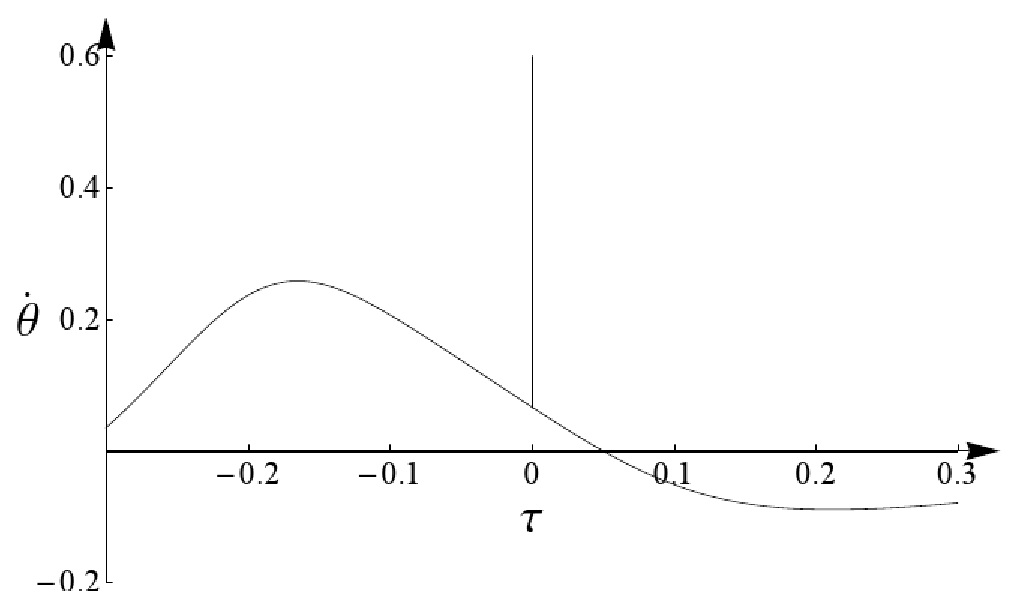
\includegraphics[width=0.45\textwidth]{singpass}
 \caption{\label{fig:singpass}
The blue trajectory passes through the singularity point
$x_{sing}=(-0.44, 3.23, -0.034, 6.37, 2.34)$ in the slice normal to
$(-0.45, -1.05, 0.3, 0.5, 0.)$. Notice how there is the gap in the
trajectory, this corresponds to the jump cause by passing through the
singularity. The red trajectory has initial point differing from the
blue's by $(0,0,0.1,0,0)$, so it does not pass through a singularity. The
green trajectory is the group orbit of $x_{sing}$ between the two
$\gSpace$ that rotate $v(x_{sing})$ in the slice. Notice how, as
predicted, the red trajectory begins near the blue trajectory, closely
follows the green trajectory after the singularity point, reaches the
other side of the blue trajectory and begins to follow it
again.
 }%
 \end{figure}


%
% ****** End of file singul.tex ******
